\documentclass{beamer}
\setbeamertemplate{bibliography item}{}
\usepackage[utf8]{vietnam}
\usepackage{amsmath}
\usepackage{amsfonts}
\usepackage{amssymb}
\usepackage{textpos}
\usepackage{enumerate}
\usepackage{graphicx}
\usepackage{booktabs}
\usepackage{cite}
\usepackage{natbib}
\usetheme{Warsaw}
\newtheorem{dn}{Định nghĩa}[section]
\newtheorem{dl}{Định lý}[section]
\newtheorem{tc}{Tính chất}[section]
\newtheorem{hq}{Hệ quả}[section]
\newtheorem{bd}{Bổ đề}[section]
\newtheorem{md}{Mệnh đề}[section]
\newtheorem{vd}{Ví dụ}[section]
\newtheorem{nx}{Nhận xét}[section]
\newcommand{\dom}{\text{{\rm dom}}}
\newcommand{\epi}{\text{{\rm epi}}}
\newcommand{\Min}{\text{{\rm Min}}}
\setbeamertemplate{theorems}[numbered]
\setbeamertemplate{definitions}[numbered]
\setbeamertemplate{footline}[frame number]
\usepackage{algorithm}
\usepackage{color}
\usepackage{algorithmic}
\usepackage{footmisc}
%\usepackage{enumitem}
\usepackage{indentfirst} 
\usepackage{comment}
\renewcommand{\thefootnote}{\arabic{footnote}}
\usefonttheme{professionalfonts}
\setbeamercolor{normal text}{bg=white,fg=black}
\renewcommand{\thefootnote}{\arabic{footnote}}
%kt
\mode<presentation>
{
 \usetheme{Darmstadt}
%\usetheme{Rochester}
}
\beamertemplatetransparentcoveredhigh

\begin{document}
\title[]{\fontsize{13pt}{10pt}\selectfont {\bf \LARGE   Phương pháp giải bài toán \\Tối ưu tuyến tính chứa tham số}\\
------------------------------------------

{\small Hướng dẫn: PGS.TS. Tạ Quang Sơn}} 
\author[]{\bf Thực hiện : NGUYỄN THÀNH NAM \& LÊ ĐỨC ANH \\
Sinh viên lớp: DTU1221, Khóa: 22}
\institute[Báo cáo luận văn thạc sĩ]{\fontsize{2pt}{2pt}}%
\small{\date{\today}}
\begin{frame}
\begin{center}
{\fontsize{8pt}{8pt}\selectfont \bf{ỦY BAN NHÂN DÂN THÀNH PHỐ HỒ CHÍ MINH\\
TRƯỜNG ĐẠI HỌC SÀI GÒN}}
\end{center}
\begin{center}
\end{center}

\begin{center}
{\fontsize{10pt}{6pt}\selectfont \bf{BÁO CÁO ĐỀ CƯƠNG NGHIÊN CỨU KHOA HỌC\\
NGÀNH: TOÁN ỨNG DỤNG}}
\end{center}
\titlepage
\end{frame}
\begin{frame}
    \frametitle{NỘI DUNG BÁO CÁO}
    \tableofcontents
\end{frame}

\section{Mục đích nghiên cứu}

\begin{frame}{Mục đích nghiên cứu}
    $\bullet$ Tối ưu tuyến tính là một nội dung quan trọng trong chương trình đào tạo Cử nhân Toán ứng dụng. Kiến thức về lý thuyết, phương pháp giải bài toán tối ưu tuyến tính đã được cung cấp cho sinh viên Khoa Toán-Ứng dụng. 
    
    $\bullet$ Với kiến thức đó, trong đề tài nghiên cứu này sẽ tìm hiểu và mở rộng thêm về dạng bài toán mà trong đó sẽ có tham số nhiễu lên bài toán Tối ưu tuyến tính được gọi là Tối ưu tuyến tính chứa tham số. 
\end{frame}
%bo
\begin{frame}{Ví dụ 1}
$\bullet$ Cho bài toán tối ưu tuyến tính như sau:

\begin{center}
    $\left(P\right)$ \quad$f(x)=-x_1+2x_2 \quad \longrightarrow $Min
\end{center}
\[\left\{\begin{aligned}
    x_1+x_2 \geq 1\\
    -x_1+x_2\leq 1\\
    x_1,x_2\geq 0
\end{aligned}\right.\]




 
\end{frame}
%bo
\begin{frame}{Ví dụ 1}
   \begin{center}
        \begin{figure}[ht]
            \begin{center}

            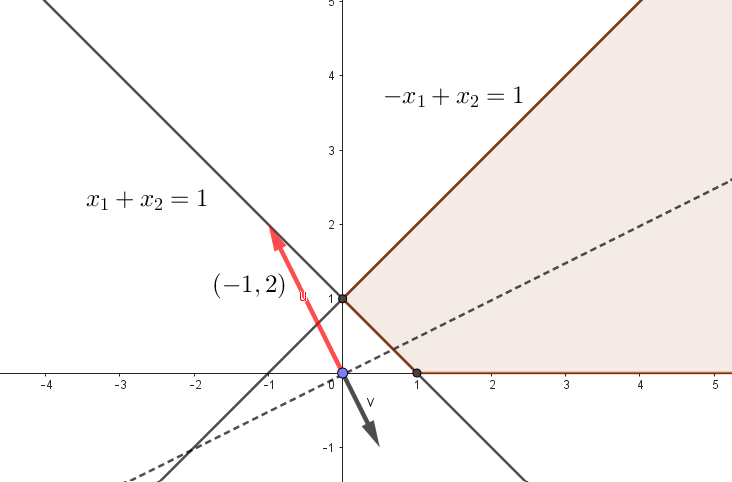
\includegraphics[width=0.75\linewidth]{hinhanh/anh1vidu1.png}  
            
            Hình minh hoạ bài toán
            \end{center}
      \end{figure}
      \end{center}

      Hướng di chuyển đường mức của bài toán tìm Min ở trên làm cho hàm mục tiêu không bị chặn và không có giá trị tối ưu.
\end{frame}


\begin{frame}{Ví dụ 1}
 Lúc này, với mong muốn bài toán có nghiệm, ta sẽ nhiễu  bằng cách thay đổi hàm mục tiêu. Giả sử với bài toán trên, ta thay đổi hệ số của nó đi một chút:
 \[\begin{aligned}
     f(x)=-x_1+2x_2 \longrightarrow f(x)=x_1+2x_2
 \end{aligned}\]
\begin{center}
     Khi đó ta vẽ lại hình minh họa
\end{center}


    

\end{frame}

\begin{frame}{Ví dụ 1}
    \begin{center}
        \begin{figure}[ht]
            \begin{center}

            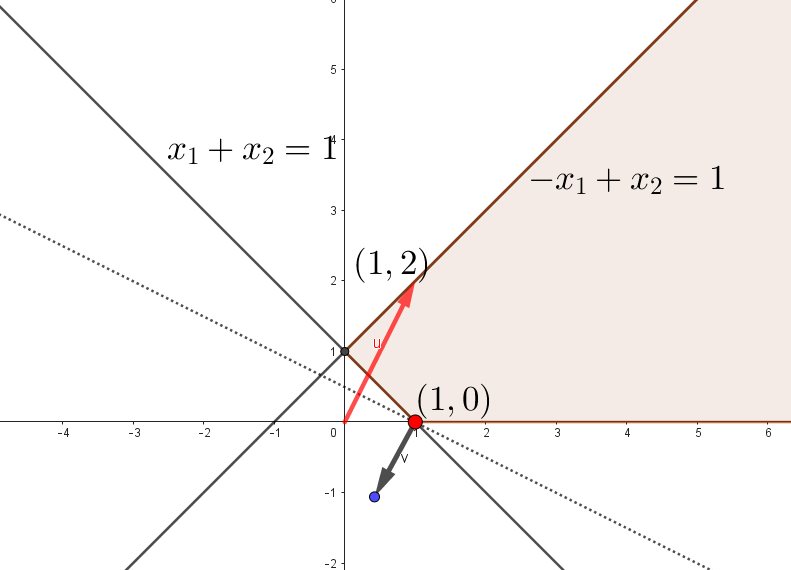
\includegraphics[width=0.75\linewidth]{hinhanh/anh3vidu1.png}  
            
            Hình minh hoạ bài toán
            \end{center}
      \end{figure}
      Dễ thấy bài toán đạt tối ưu tại điểm $(1;0)$
      \end{center}
      
\end{frame}


\begin{frame}{Ví dụ 2}

Một nhà máy sản xuất hai sản phẩm trên 2 máy:

\begin{itemize}
    \item Đơn vị sản phẩm I cần 2 giờ trên máy 1 và 1 giờ trên máy 2.
    \item Đơn vị sản phẩm II cần 1 giờ trên máy 1 và 3 giờ trên máy 2.
    \item Doanh thu lần lượt cho từng đơn vị sản phẩm I,II là 30USD và 20USD.
    \item Thời gian làm việc tối thiểu của mỗi máy là 8 giờ.
\end{itemize}
Hãy tìm số đơn vị sản phẩm để thu được lợi nhuận cao nhất.

\end{frame}
 \begin{frame}{Ví dụ 2}
     Ta có bài toán tối ưu tuyến tính như sau
     \begin{center}
            $\left(P\right)$ $f(x)=30x_1+20x_2 \longrightarrow$Max
     \end{center}
  \[\left\{\begin{aligned}
      2x_1+x_2\leq 8\\
      x_1+3x_2\leq 8\\
      x_1,x_2\geq 0
  \end{aligned}\right.\]
\begin{center}
    Ta thu được nghiệm tối ưu của bài toán này là $(3.2,1.6)$ 
     
\end{center}

 \end{frame}
    
\begin{frame}{Ví dụ 2}
    \begin{center}
        \begin{figure}
            
            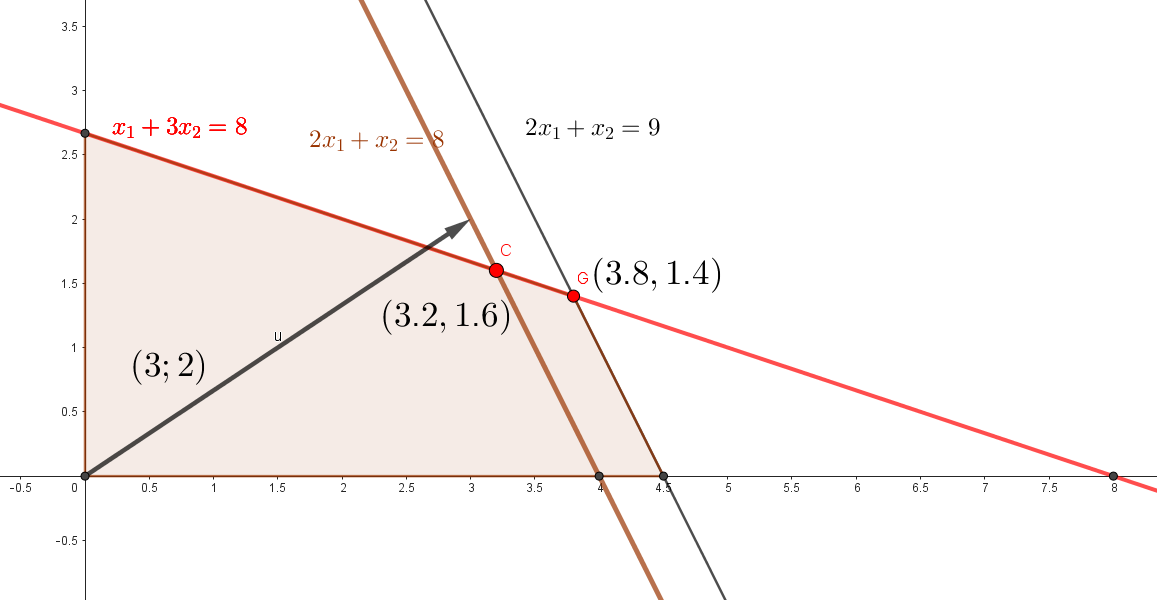
\includegraphics[width=0.8\linewidth]{hinhanh/anh2vidu2.png}
      
        \end{figure}
        Hỉnh minh họa cho bài toán
    \end{center}
    
\end{frame}

\section{Nội dung nghiên cứu}
\begin{frame}{Nội dung nghiên cứu}
    \begin{itemize}
    \item Hệ thống lại cơ sở lý thuyết và phương pháp giải các bài toán Tối ưu tuyến tính.
    \item Từ đó mở rộng để tìm hiểu về bài toán tối ưu tuyến tính có tham số thông qua 2 dạng bài toán:
    \begin{itemize}
    \item Tối ưu tuyến tính có tham số ở hàm mục tiêu.
    \item Tối ưu tuyến tính có tham số ở vế phải của ràng buộc.
    \end{itemize}
    \end{itemize}
\end{frame}
\section{Dự kiến nội dung đề tài}
\begin{frame}{Dự kiến nội dung đề tài}
    \begin{itemize}
    \item Chương 1:  Bao gồm các kiến thức chuẩn bị, nội dung có liên quan đến
    một số kiến thức cơ bản của quy hoạch tuyến tính để dùng
    làm cơ sở nghiên cứu về các phương pháp giải của bài toán tối ưu tuyến tính có tham số.
    \item Chương 2: Tìm hiểu về các phương pháp và thuật giải giúp giải quyết bài toán Tối ưu tuyến tính có tham số ở hàm mục tiêu và Tối ưu tuyến tính có tham số vế phải của ràng buộc.
    \item Chương 3: Một số ví dụ áp dụng của bài toán tối ưu tuyến tính có tham số vào các bài toán cụ thể .
    \end{itemize}   
\end{frame}
\section{Tổ chức và phân công}
\begin{frame}[shrink=20]
    \frametitle{Tổ chức và phân công}
    \vspace{1.5cm}
    \begin{table}
        \begin{tabular}{|p{2.5in}|c|c|}
            \hline
            \textbf{Nội dung} & Người phụ trách chính & Người cộng tác \\
            \hline \hline
            \textbf{Chương 1} && \\
            \hline
            Cơ sở lý thuyết quy hoạch tuyến tính & Nguyễn Thành Nam & \\
            & Lê Đức Anh & \\
            \hline
            \textbf{Chương 2} && \\
            \hline
           Tối ưu tuyến tính có tham số hàm mục tiêu & Nguyễn Thành Nam & Lê Đức Anh \\
           \hline
           Tối ưu tuyến tính có tham số vế phải của ràng buộc & Lê Đức Anh & Nguyễn Thành Nam\\
            \hline
            \textbf{Chương 3} && \\
            \hline
            Các bài toán ứng dụng & Nguyễn Thành Nam & \\
            & Lê Đức Anh & \\
            \hline
        \end{tabular}
    \end{table}
\end{frame}
\section{Tiến độ thực hiện}
\begin{frame}{Tiến độ thực hiện}
Thời gian nghiên cứu chia làm 3 giai đoạn:
\begin{itemize}
\item Giai đoạn 1 (? tháng): Đọc, hiểu tài liệu liên quan đến lý thuyết tối ưu tuyến tính có tham số và các phương pháp giải.
\item Giai đoạn 2 (? tháng): Thu hoạch, hệ thống lại các tri thức và viết luận văn.
\item Giai đoạn 3 (? tháng): Hoàn thành và bảo vệ luận văn.
\end{itemize}
\end{frame}


\section{Tài liệu tham khảo}
  \begin{frame}{Tài liệu tham khảo}
\begin{thebibliography}{xxx}
%1%
\bibitem{T}   Tạ Quang Sơn, Bài giảng Quy hoạch tuyến tính, Đại học Sài Gòn, 2023.

\bibitem{E} Elementary Linear Programming with Applications (1995, Academic Press).
%2%
\bibitem{H} Hu T.C.-Linear and Integer Programming Made Easy.
\bibitem{L} Linear Programming - Foundations and Extensions - Springer US (2001).
\bibitem{B}Bùi Phúc Trung, Nguyễn Thị Ngọc Thanh, Vũ Thị Bích Liên, Giáo trình Quy hoạch tuyến tính Tối ưu hóa-NXB Lao Động-Xã Hội-2003
NXB Lao Động-Xã Hội-2003.

\end{thebibliography}
\end{frame}
\begin{frame}\frametitle{Kết thúc}
\begin{block}{}
\medskip
\center{\huge \it \textcolor[rgb]{0.50,0.30,1.0}{Cảm ơn quý thầy cô và các anh chị đã quan tâm theo dõi!}}
\medskip
\end{block}	
\end{frame}
\end{document}

